%%%%%%%%%%%%%%%%%%%%%%%%%%%%%%%%%%%%%%%%%
% Beamer Presentation
% LaTeX Template
% Version 1.0 (10/11/12)
%
% This template has been downloaded from:
% http://www.LaTeXTemplates.com
%
% License:
% CC BY-NC-SA 3.0 (http://creativecommons.org/licenses/by-nc-sa/3.0/)
%
%%%%%%%%%%%%%%%%%%%%%%%%%%%%%%%%%%%%%%%%%
% Adapted by Daniel Alexander from Meenakshi Sundaram's presentation of the same title
%----------------------------------------------------------------------------------------
%	PACKAGES AND THEMES
%----------------------------------------------------------------------------------------

\documentclass{beamer}

\mode<presentation> {

% The Beamer class comes with a number of default slide themes
% which change the colors and layouts of slides. Below this is a list
% of all the themes, uncomment each in turn to see what they look like.

%\usetheme{default}
%\usetheme{AnnArbor}
%\usetheme{Antibes}
%\usetheme{Bergen}
%\usetheme{Berkeley}
%\usetheme{Berlin}
%\usetheme{Boadilla}
\usetheme{CambridgeUS}
%\usetheme{Copenhagen}
%\usetheme{Darmstadt}
%\usetheme{Dresden}
%\usetheme{Frankfurt}
%\usetheme{Goettingen}
%\usetheme{Hannover}
%\usetheme{Ilmenau}
%\usetheme{JuanLesPins}
%\usetheme{Luebeck}
%\usetheme{Madrid}
%\usetheme{Malmoe}
%\usetheme{Marburg}
%\usetheme{Montpellier}
%\usetheme{PaloAlto}
%\usetheme{Pittsburgh}
%\usetheme{Rochester}
%\usetheme{Singapore}
%\usetheme{Szeged}
%\usetheme{Warsaw}

% As well as themes, the Beamer class has a number of color themes
% for any slide theme. Uncomment each of these in turn to see how it
% changes the colors of your current slide theme.

%\usecolortheme{albatross}
%\usecolortheme{beaver}
%\usecolortheme{beetle}
%\usecolortheme{crane}
%\usecolortheme{dolphin}
%\usecolortheme{dove}
%\usecolortheme{fly}
%\usecolortheme{lily}
%\usecolortheme{orchid}
%\usecolortheme{rose}
%\usecolortheme{seagull}
%\usecolortheme{seahorse}
%\usecolortheme{whale}
%\usecolortheme{wolverine}

%\setbeamertemplate{footline} % To remove the footer line in all slides uncomment this line
%\setbeamertemplate{footline}[page number] % To replace the footer line in all slides with a simple slide count uncomment this line

%\setbeamertemplate{navigation symbols}{} % To remove the navigation symbols from the bottom of all slides uncomment this line
%\setbeamercovered{invisible}
}

%\AtBeginSection[] {
%    \begin{frame}%[plain]
%    \frametitle{Overview}
%    \tableofcontents[currentsection]
%  \end{frame}
%} 

\usepackage{graphicx} % Allows including images
\usepackage{booktabs} % Allows the use of \toprule, \midrule and \bottomrule in
\usepackage{amsmath}
\usepackage{amsfonts}
\usepackage{amssymb}
\usepackage[final]{showexpl}
%----------------------------------------------------------------------------------------
%	TITLE PAGE
%----------------------------------------------------------------------------------------

\title[\LaTeX]{Introduction to \LaTeX} % The short title appears at the 
%bottom of every slide, %the full title is only on the title page

\author{Daniel Alexander} % Your name
\institute[CISER] % Your institution as it will appear on the 
%bottom of every slide, may be shorthand to save space
{
CISER, Cornell University \\ % Your institution for the title page
\medskip
\textit{dra65@cornell.edu} % Your email address
}
\date{Feb 18$^{th}$ 2019} % Date, can be changed to a custom date

\begin{document}

\begin{frame}
\titlepage % Print the title page as the first slide
\end{frame}

\begin{frame}
\frametitle{Overview} % Table of contents slide, comment this block out to remove it
\tableofcontents % Throughout your presentation, if you choose to use \section{} and \subsection{} commands, these will automatically be printed on this slide as an overview of your presentation
\end{frame}

%----------------------------------------------------------------------------------------
%	PRESENTATION SLIDES
%----------------------------------------------------------------------------------------

%------------------------------------------------
\section{Broad Overview} 
\begin{frame}{Elements of Digital Publishing}
 The elements of publishing:
 \begin{itemize}
 \item \textbf{Layout design}
 \begin{itemize}
  \item Font size
  \item Spacing
  \item Margins
  \item Column width
  \item Headings
  \item $\cdots$
 \end{itemize}
 %\pause
 \item \textbf{Typesetting}
 \begin{itemize}
  \item Organizing content according to layout
 \end{itemize}
\end{itemize}
\end{frame}

\begin{frame}{\TeX{} and \LaTeX}
 \begin{columns}[t]
  \column{.45\textwidth}
  
  \begin{center}
    {\large \TeX}
    \begin{block}{Developer: Donald E. Knuth}
     \centering
     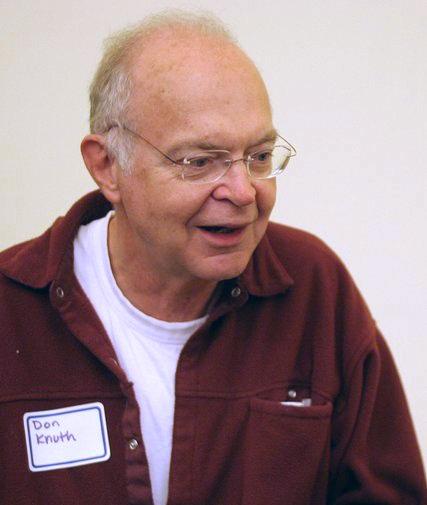
\includegraphics[height=0.2\textheight]{pics/Knuth.jpg}
    \end{block}
    {\tiny
    \begin{itemize}
    \item Year: 1978
    \item Current Version: 3.14159265
    \item Typesetting engine for digital printing
    \item Pronounced: ``Tech''
    \item Renowned for stability
    \end{itemize}
    }
  \end{center}
  
  %\pause
  \column{.45\textwidth}
  
  \begin{center}
    {\large \LaTeX}
    \begin{block}{Developer: Leslie Lamport}
     \centering
      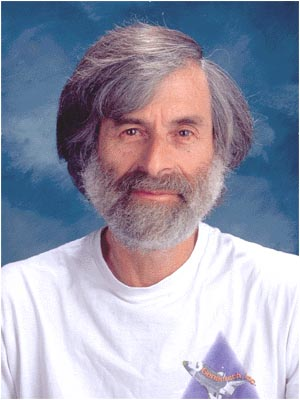
\includegraphics[height=0.20\textheight]{pics/Leslie_Lamport.jpg}
    \end{block}
    {\tiny
    \begin{itemize}    
    \item Year: 1980
    \item Current Version: \LaTeXe
    \item Document Preparation System  
    \item Pronounced: ``Lay Tech''
    \item Uses \TeX{} for typesetting
    \item Composed of \TeX{} macros
    \end{itemize}
    }
    \end{center}
 \end{columns}
\end{frame}

\begin{frame}{Elements of Digital Publishing}
 \begin{columns}
  \column{.45\textwidth}
  The elements of publishing:
  \begin{itemize}
   \item {\color{blue}\textbf{Layout design}}
   \begin{itemize}
   {\color{blue}
     \item Font size
     \item Spacing
     \item Margins
     \item Column width
     \item Headings
     \item $\cdots$}
   \end{itemize}   
   \item {\color{red}\textbf{Typesetting}}
   \begin{itemize}
     \item {\color{red}Organizing content according to layout}
   \end{itemize}
   \end{itemize}
   \column{.45\textwidth}
   \begin{itemize}
   \item {\color{blue}{\Large \LaTeX}}
   \end{itemize}
   \vspace{2.5cm}
   \begin{itemize}
   \item {\color{red}{\Large \TeX}}
   \end{itemize}
 \end{columns}
\end{frame}


\begin{frame}
\frametitle{\LaTeX{} Vs WYSIWYG word processors}

The gap between WYSIWYG word processors and \LaTeX{} is closing down. 
\vspace{1cm}
%\pause
\begin{columns}[t]
 \column{0.5\textwidth}
\textbf{WYSIWYG word processors}:
\begin{itemize}
 \item Collaborative editing
 \item Spell check
 \item Compatibility
 \item Low Learning Curve
\end{itemize}
%\pause
\column{0.5\textwidth}
\textbf{\LaTeX{}}:
\begin{itemize}
  \item Consistent intradocument referencing 
  \item Clean mathematical notation
  \item Separation of content and style
  \item Clean tables and illustration
\end{itemize}
\end{columns}
\end{frame}

\section{Your first \LaTeX{} document}

\begin{frame}[fragile]{Compiling}

\begin{itemize}
  \item Implementation of \LaTeX{}, \TeX{} opensource domain. 
  \begin{itemize}
  \item Windows users --- MiK\TeX 
  \item Linux users --- Precompiled Binaries
  \item Mac users --- Mac\TeX{}, Xe\LaTeX
  \end{itemize}
\end{itemize}
%\pause
\begin{itemize}
 \item Input to \LaTeX{} --- plain text file containing:
 \begin{itemize}
 \item Content of the document
 \item Instructions on typesetting
 \end{itemize}
\end{itemize}
%\pause
Typically the process of conversion from the plain text file into a pdf 
document happens through a program called `pdflatex' using the underlying 
implementation.
 %\pause
 \begin{figure}
  \centering
  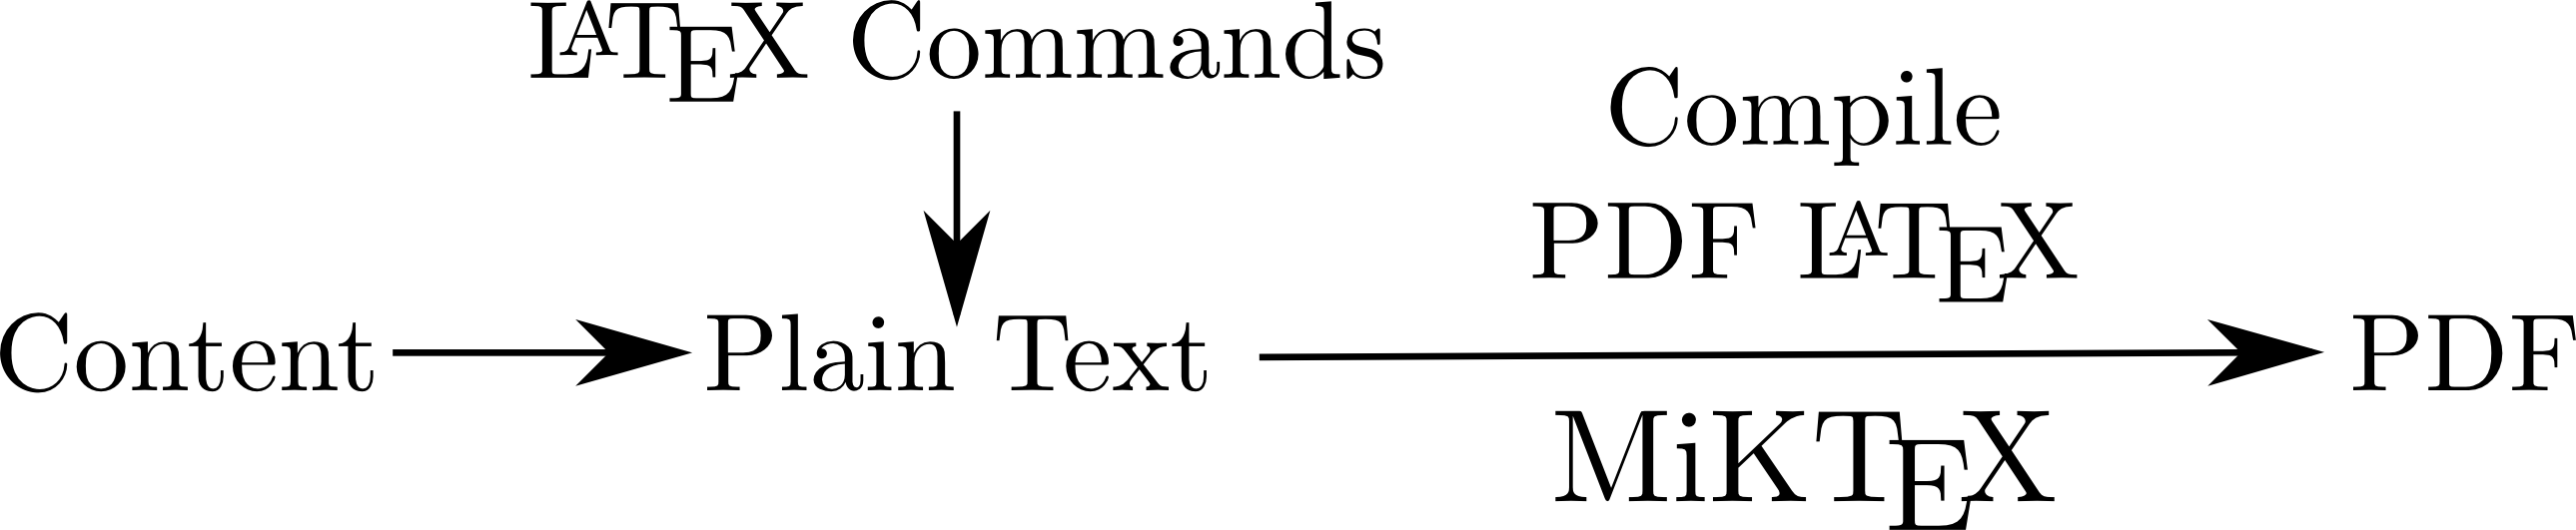
\includegraphics[scale=0.4]{pics/Compiling.png}
 \end{figure}
\end{frame}

\begin{frame}{Integrated Development Environment}

Typically all packaged into an Integrated Development Environment (IDE).

\begin{itemize}
 \item \TeX nicCenter - \url{http://www.texniccenter.org/}
 \item \TeX works - \url{https://www.tug.org/texworks/}
 \item Winedit - \url{http://www.winedt.com/}
 \item \TeX maker - \url{http://www.xm1math.net/texmaker/}
 \item LEd - \url{http://www.latexeditor.org/}
 \item Kile - \url{http://kile.sourceforge.net/}
\end{itemize}

Online IDE
\begin{itemize}
 \item Overleaf - \url{https://www.overleaf.com/}
 \item Share\LaTeX{} - \url{https://www.sharelatex.com/}
\end{itemize}

\begin{block}{Note}
Minimum requirement is only a plain text file with content, commands 
and a \LaTeX{} installation to get an output.
\end{block}

\end{frame}

\begin{frame}[fragile]{Example 1: Washing Dishes to Wash Them}
 
 \begin{itemize}
  \item Use the IDE in your computer/web. 
  \item Open/Upload the \TeX{} file and allied files in folder `example1'.
  \item Set your compiler to pdflatex.
  \item Compile it to get your output. 
 \end{itemize}
\end{frame}
 
\begin{frame}[fragile]{Example 1: Washing Dishes to Wash Them}
 \begin{figure}
 \centering
 \includegraphics[height=0.3\textheight]{pics/washingdishes.jpg} 
 \end{figure}
 %\pause
\begin{columns}[t]
\column{0.7\textheight}
\begin{block}{Example 1}
\tiny
\begin{verbatim}
\documentclass[a4paper,12pt]{article}
\title{Washing the dishes to wash the dishes}
\author{Thich Nhat Hanh}
\usepackage{graphicx}
\begin{document}
 \maketitle
\begin{center}
\includegraphics[scale=0.25]{washingdishes.jpg}
\end{center}
Thirty years ago ...........
and we are incapable of actually living one 
minute of life.
\end{document}
\end{verbatim}
\end{block}
\end{columns}
\end{frame}

\section{Somethings about the Language}
\begin{frame}[fragile]{Spaces, Breaks, and Special Char}

\begin{block}{Space, Line Breaks, Paragraph breaks, }
``Whitespace'' characters such as blank and tab are treated as a
``space''. A ``\textbackslash \textbackslash{}'' is a line break. An empty line 
between two text streams is a paragraph break.
\end{block}
%\pause
{\tiny
\begin{LTXexample}
It does not matter whether you enter one or 
several     spaces after a word it is still
treated\\ as a single space.


It does not matter whether you have one or 
more empty lines, it is still treated as a 
new paragraph.
\end{LTXexample}
}
%\pause
\begin{block}{Special Characters}
Reserved Characaters \# \$ \% \^{} \& \_ \{ \} \~{} 
\textbackslash
\end{block}
%\pause
{\tiny
\begin{LTXexample}
\# \$ \% \^{} \& \_ \{ \} \~{} \textbackslash
\end{LTXexample}
}
\end{frame}

\begin{frame}[fragile]{Commands and Comments}
\begin{block}{\LaTeX{} commands}
 \centering
\textbackslash \textsl{command}[\textsl{optional 
parameter}]\{\textsl{parameter}\}
\end{block}
%\pause
{\tiny
\begin{LTXexample}
\TeX{} and \LaTeX \newline
\underline{Underline}, \textit{Italics} and \textbf{Bold} \newline
\today \newline
\end{LTXexample}
}
%\pause
\begin{block}{Comments}
 The \% sign is used to mark single line comments.
\end{block}
%\pause
{\tiny
\begin{LTXexample}
This is an % stupid
% Better: instructive <----
example: Supercal%
              ifragilisticexpialidocious
\end{LTXexample}
}
\end{frame}

\begin{frame}[fragile]{Example 2: Washing the Dishes to Wash Them}
Open the \TeX{} file in folder example2. 

The second paragraph is a continuation 
of the same thought so replace the paragraph break with a line 
break.
%\pause

{\tiny
\begin{LTXexample}
 \ldots one hundred monks.
\\
There was no soap \ldots
\end{LTXexample}
}
%\pause

Notice the change in the indentation from paragraph breaks. Now convert the 
following text to boldface: ``At first glance, that might seem a little 
silly \ldots like a bottle slapped here and there on the waves.''
%\pause

{\tiny
\begin{LTXexample}
 \textbf{At first glance, that might seem a little 
silly:\ldots like a bottle slapped here 
and there on the waves.}
\end{LTXexample}
}
%\pause

Convert the last paragraph to italics.
%\pause

{\tiny
\begin{LTXexample}
 \textit{In fact we are completely incapable
 of realizing the miracle of life 
\ldots and we are incapable of
actually living one minute of life. }
\end{LTXexample}
}
\end{frame}

\section{Document Structure}
\begin{frame}[fragile]{Document Structure}
\begin{block}{\textbackslash documentclass[$\langle$ Options 
$\rangle$]\{Type of Document\}}
\tiny
 What class of document? article, report, book, beamer, memoir, 
letter, etc. \\
 What options? 10pt, 12pt, a4paper, a3paper, landscape, portrait, twocolumn,  
etc.
\end{block}
%\pause
{\tiny Commands that affect the entire document. Declare new 
environemnts, commands, and add packages to provide additional features.\par}
%\pause
\begin{block}{\textbackslash usepackage[$\langle$ Options $\rangle$]\{Package 
name\}}
\tiny

Examples: \textbackslash usepackage\{graphicx\}, \textbackslash 
usepackage\{titlepic\}, \textbackslash usepackage[hidelinks]\{hyperref\}, etc.
\end{block}
%\pause
{\tiny After all setup we start the body of the text with this command.}
%\pause
\begin{block}{\textbackslash begin\{document\}}
\tiny
Write content with logical demarkations such as \textbackslash 
maketitle, \textbackslash chapter\{title\}, \textbackslash part\{title\},  
\textbackslash section\{title\}, 
\textbackslash subsection\{title\},etc.
\\ Use environments such as \textbackslash begin\{abstract\} \ldots 
\textbackslash 
end\{abstract\}, \textbackslash begin\{equation\} \ldots 
\textbackslash 
end\{equation\}, \textbackslash begin\{itemize\} \ldots \textbackslash 
end\{itemize\}, \textbackslash begin\{enumerate\} \ldots \textbackslash 
end\{enumerate\}, etc.
\end{block}

\begin{block}{\textbackslash end\{document\}}
\tiny
Marks the end of the content. 
\end{block}
\end{frame}

\begin{frame}[fragile]{Example 3: A Guide To Walking Meditation}
You are given a \TeX{} document in the folder ``example3'' that has only the 
content. Let us add the structural component and compile it.
\begin{figure}
\centering
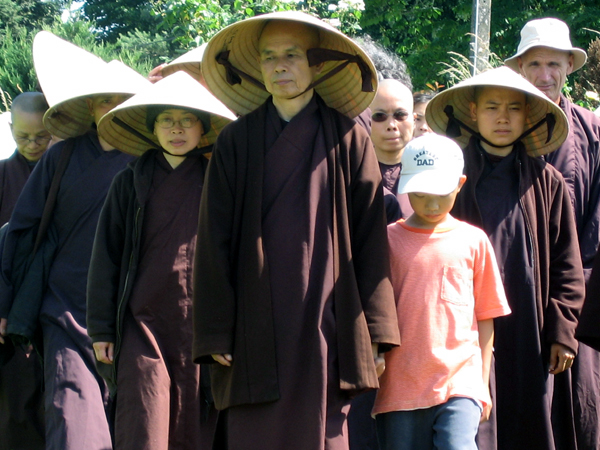
\includegraphics[height=0.2\textheight]{pics/walkingmeditation.jpg}
\end{figure}
%\pause
%\pause
\begin{columns}[t]
\column{0.45\textwidth}
\begin{block}{Structural Components}
 \tiny
 \begin{itemize}
 \item Declare the nature of the document with options
 \item Identify the title and the author
 \item Start the document environment
 \item Make the title
 \item Identify Sections and other logical subdivisions.
 \item End the document environment
\end{itemize}
\end{block}
%\pause

\column{0.45\textwidth}
\begin{block}{Structural Components}
\tiny
\begin{verbatim}
 \documentclass[a4paper,12pt,twocolumn]{article}
 \title{A Guide to Walking Meditation}
 \author{Thich Nhat Hanh}
 \begin{document}
 \maketitle
 \section{Your Steps Are Most Important}
 .
 .
 .
 \end{document}
\end{verbatim} 
\end{block}
 
\end{columns}

\end{frame}


\section{Environments}

\begin{frame}[fragile]{Environments}

\begin{block}{\textbackslash begin\{ \ldots \} \ldots \textbackslash 
end \{ \ldots \} }
These are logical structures within the document. It is established by a 
``begin'' and an ``end'' statement.
\end{block}
%\pause
Let us see some examples
\end{frame}

\begin{frame}[fragile]{Environments: Itemize}


\begin{block}{Itemize}
 \tiny
\begin{verbatim}
 \begin{itemize}
  \item 
  \item
  \item
 \end{itemize}
\end{verbatim} 

\begin{LTXexample}
Funny ones from \url{www.dearblankpleaseblank.com}
 \begin{itemize}
  \item  Dear Noah, \\
  We could have sworn you said 
  the ark wasn't leaving till 5. \\
  Sincerely, \\
  Unicorns 
  \item  Dear Icebergs,\\
  Sorry to hear about the global 
  warming. Enjoy the Karma\ldots \\
  Sincerely,\\
  The Titanic. 
  \item Dear Rubik's Cube,\\
  Done!\\
  Sincerely,\\
  Colorblind 
 \end{itemize}
\end{LTXexample}

\end{block}

\end{frame}

\begin{frame}[fragile]{Environments: Enumerate}
\begin{block}{Enumerate}
 \tiny
\begin{verbatim}
 \begin{enumerate}
  \item 
  \item
  \item
 \end{enumerate}
\end{verbatim} 

\begin{LTXexample}
Funny ones from \url{www.dearblankpleaseblank.com}
 \begin{enumerate}
  \item  Dear Noah, \\
  We could have sworn you said 
  the ark wasn't leaving till 5. \\
  Sincerely, \\
  Unicorns 
  \item  Dear Icebergs,\\
  Sorry to hear about the global 
  warming. Enjoy the Karma\ldots \\
  Sincerely,\\
  The Titanic. 
  \item Dear Rubik's Cube,\\
  Done!\\
  Sincerely,\\
  Colorblind
 \end{enumerate}
\end{LTXexample}
\end{block}
\end{frame}

\begin{frame}[fragile]{Environments: Figures}
\begin{itemize}
\item Inserting figures needs an addon package \--- \textbackslash 
usepackage\{graphicx\} added in the \textit{preamble} before the \textbackslash 
 begin\{document\} environment.
 \item For inline figures i.e., ones that flows with text use the 
following command.
\begin{block}{Inline Figures}
\tiny
\begin{verbatim}
\includegraphics[<Options>]{path to figure}
\end{verbatim}
\end{block}
%\pause
\item For floating figures i.e., ones that float around with text adjusted 
accordingly use the following environment and the command
\begin{block}{Floating Figures}
\tiny
\begin{verbatim}
\begin{figure}[location options]
    \includegraphics[<Options>]{path to figure }
    \caption{ text }
\end{figure}
\end{verbatim}
\end{block}
\end{itemize}
\end{frame}

\begin{frame}[fragile]{Environments: Figures}
\begin{itemize}
 \item Figure Options
\begin{itemize}
\item Options for figure placement
\begin{itemize}
\item ! \--- ignore \TeX{} algorithms
\item h \--- place the figure here
\item t \--- place the figure on the top of the page
\item b \--- place the figure at the bottom of the page
\item p \--- place graphics in a new page alltogether
\end{itemize}
\item Provide multiple options
\item Failure of location suggestion implies difficulty with layout and text
\end{itemize} 
\item includegraphics options
\begin{itemize}
\item scale \--- scales a figure ex: scale=0.5
\item width \--- changes the width of the figure ex: width=5cm
\item height \--- changes the height of the figure ex: height=5cm
\end{itemize}
\end{itemize}
\end{frame}

\begin{frame}[fragile]{Example 4: Stir Frying Spinach}
Open the given \TeX{} document in folder ``example4''. In this document you are to incorporate a picture named ``stirfryspinach.jpg'' in the 
beginning of the document after the title.

%\pause

\begin{columns}
\column{0.5\textwidth}
\begin{block}{Example 4}
\tiny
In the preamble insert 
\begin{verbatim}
\usepackage{graphicx}
\end{verbatim}
After the command \textbackslash maketitle insert the following snippet
\begin{verbatim}
  \begin{figure}[h]
   \includegraphics[scale=0.5]{stirfryspinach.jpg}
  \end{figure}
 \end{verbatim}
\end{block}
%\pause
\column{0.5\textwidth}
\begin{figure}
 \centering
 \includegraphics[height=0.25\textheight]{pics/stirfryspinach.jpg}
\end{figure} 
\end{columns}
 %\pause 

 \vspace{0.5cm}

 You are to now \textit{itemize} the contents of every section except the 
section titled ``Procedure'' which needs to be \textit{enumerated}.
\end{frame}

\section{Math}
\begin{frame}[fragile]{Inline and display math}
\begin{itemize}
 \item Inline \$ {\color{red} math content} \$.
 %\pause
{\tiny
\begin{LTXexample}
Represent $a$ divided by $b$?
It is $\frac{a}{b}$.

What is $2^4$?
It is $16$.

What is $\sin(\phi+\theta)$?
It is $\sin(\theta)\cos(\phi)+
\sin(\phi)\cos(\theta)$.
\end{LTXexample}
}
%\pause
\item Displayed math content in a separate line. 
\begin{itemize}
\tiny
\item \textbackslash begin\{equation\} \ldots \textbackslash end \{equation\}
\item \textbackslash begin\{equation*\} \ldots \textbackslash end \{equation*\} 
\end{itemize}
\item Packages needed
\begin{itemize}
\tiny
\item amsmath, amssymb, amsfont
\end{itemize}
%\pause
{\tiny
\begin{LTXexample}
\begin{equation*}
 \int_{a}^{b} x dx 
 = \frac{b^2-a^2}{2}
\end{equation*}

\begin{equation}
 a\left(\frac{\partial \sigma^2y}
 {\partial y}\right)
 = a\sigma^2
\end{equation}

\end{LTXexample}
}
\end{itemize}
\end{frame}

\begin{frame}[fragile]{Elements of Math Mode}
\begin{itemize}
\item Greek letters
\item Exponents, superscripts, and subscripts
\item Nth root and surds
\item Dots 
{\tiny
\begin{LTXexample}
\begin{equation*}
\alpha, \beta, \gamma, \phi, \theta 
\end{equation*}
\begin{equation*}
a^b, a_b, a^{b_c}_{d^e}
\end{equation*}
\begin{equation*}
\sqrt[n]{ax^2+bx+c},\sqrt{gtx}, \surd{x}
\end{equation*}
\begin{equation*}
 \Psi=v_1 \cdot v_2 \cdot \ldots 
 \qquad \vdots,\qquad \ddots
\end{equation*}
\end{LTXexample}
}
\end{itemize}
\end{frame}

\begin{frame}[fragile]{Elements of Math Mode}
\begin{itemize}
\item \textbackslash underline, \textbackslash overline, \textbackslash 
overbrace, \textbackslash underbrace
\item Accents
\item Standard functions
\item Fractions
{\tiny
\begin{LTXexample}
\begin{equation*}
\underline{a}, \overline{b}, 
\overbrace{a+b+c}^q, \underbrace{d+e+f}_p
\end{equation*}
\begin{equation*}
\tilde{a},\widetilde{abc},\hat{q},
\widehat{pqr},\overrightarrow{a},
\overleftarrow{ghj}
\end{equation*}
\begin{equation*}
\sin,\cos,\arcsin,\lg,\inf,\exp,\lim,\min
\end{equation*}
\begin{equation*}
 \frac{1}{2}, 1/2, \tfrac{1}{2}
\end{equation*}
\end{LTXexample}
}
\end{itemize}
\end{frame}

\begin{frame}[fragile]{Elements of Math Mode}
\begin{itemize}
\item Integral, Product, Sum
\item Bracketing and other delimiters 
{\tiny
\begin{LTXexample}
\begin{equation*}
\int_0^{\frac{\pi}{2}}, 
\prod_{i\in \mathcal{N}},
\sum_{i=1}^{N}
\end{equation*}
\begin{equation*}
 \left(1 + \frac{a}{b}\right),
 \left[a^{\sin(x)}\right],
 \left|\left| v \right|\right| 
 \qquad \left( \because a \neq b \right.
\end{equation*}

\end{LTXexample}
}
%\pause
\item Multiline Equations 
\begin{itemize}
\tiny
\item \textbackslash begin\{align\} \ldots \textbackslash end\{align\}
\begin{LTXexample}
\begin{align}
  a & = b + c \\
  & = d + e + f + 
  g + h + i \nonumber\\
  & + m + n + o \\
  & = p + q + r + s
\end{align}
\end{LTXexample}
\end{itemize}
\end{itemize}
\end{frame}

\begin{frame}[fragile]{Example 5: Quadratic Formula}
 In this example the math content has been written in text form and we are to 
convert them into \TeX{}. Open the \TeX{} file from the folder ``example5''.

You are to correct the math content.
%\pause
\begin{columns}
 \column{0.5\textwidth}
 \begin{itemize}
 \tiny
  \item Include the package amsmath in the preamble
  \item Put in \$ \$ for inline text. 
  \item Replace ``not equal to'' with a symbol ``\textbackslash neq''.
  \item Single line equations can be put in the equation environment.
  \item Multiline equations can be put in the align environment.
  \item Use \textbackslash frac to represent fractions in the equation 
environment.
  \item Put in parantheses with \textbackslash left( and \textbackslash right).
 \end{itemize}
\end{columns}
\end{frame}

\begin{frame}[fragile]{Example 5: Quadratic Formula}
\begin{columns}
\column{0.75\textwidth}
{\tiny
\begin{verbatim}
\usepackage{amsmath}
...
For a first degree equation $ax+b=0$ with $a \neq 0$ 
the solution is $x=-b/a$.  We now look at solving $ax^2+bx+c=0$.
...
The equation $ax^2+bx+c=0$ with $a \neq 0$ has the solutions
...
\begin{equation}
x=\frac{-b \pm \sqrt{b^2-4ac}}{2a}
\end{equation}
...
We use the method of completing the square to rewrite $ax^2+bx+c$.
....
\begin{align}
ax^2+bx+c &= a \left( x^2 + \frac{b}{a} x \right)+c \\
&=a\left(x^2 + \frac{b}{a} x + \frac{b}{2a} \right)^2 -\frac{b}{2a}^2 +c\\
&=a\left(x + \frac{b}{2a}\right)^2 -  a\left(\frac{b}{2a}\right)^2+c \\
&=a\left(x+\frac{b}{2a}\right)^2 - \frac{\left(b^2-4ac\right)}{4a}.
\end{align}
Therefore $ax^2+bx+c=0$ can be rewritten as 
\end{verbatim}
}
\end{columns}
\end{frame}

\begin{frame}[fragile]{Example 5: Quadratic Formula}
\begin{columns}
 \column{0.5\textwidth}
{\tiny
\begin{verbatim}
\begin{equation}
a\left(x+\frac{b}{2a}\right)^2 - \frac{\left(b^2-4ac\right)}{4a}=0,
\end{equation}
....
\begin{equation}
\left(x+\frac{b}{2a}\right)^2= \frac{\left(b^2-4ac\right)}{4a^2}.
\end{equation}
...
\begin{equation}
x+\frac{b}{2a}= \pm \frac{\sqrt{b^2-4ac}}{2a}
\end{equation}
...
\begin{equation}
x=\frac{-b \pm \sqrt{b^2-4ac}}{2a}
\end{equation}
\end{verbatim}
}
\end{columns}
\end{frame}

\section{Referencing}
\begin{frame}[fragile]{Intradocument Referencing}
 \begin{itemize}
  \item To refer to content within a document we use the combination of 
\textbackslash label \{Key\} and \textbackslash ref \{Key\}. 
 \end{itemize}
%\pause 
 {\tiny
\let\orilabel\label
\begin{LTXexample}[frame=none,preset=\let\label\orilabel]
In Eq. \ref{eq:quad} the roots
of a generic quadratic equation
are represented.\label{sec:quad}
\begin{equation}
x=\frac{-b \pm 
\sqrt{b^2-4ac}}{2a} \label{eq:quad}
\end{equation}
Oceanic breath:
\begin{enumerate}
 \item Open your mouth.
 \item Inhale and Exhale 
 (sigh) deeply through it. 
 \item Close your mouth 
 and repeat the same action.
 \label{step:openthroat}
 \item Continue breathing 
 like this for 20 cycles.
\end{enumerate}
Step. \ref{step:openthroat} opens up your 
 throat cavity and you 
 breathe through it.
\end{LTXexample}
}
\end{frame}

\begin{frame}[fragile]{Citing}

There are many ways to cite documents in \LaTeX{}. A simple way is to use 
``thebibliography'' environment.
%\pause
\begin{block}{thebibliography}
 \begin{verbatim}
 In text one can cite using command \cite{citekey}.
 
  \begin{thebibliography}{size of widest label}
    \bibitem[label]{citekey} reference to be cited
  \end{thebibliography}
 \end{verbatim}
\end{block} 
\end{frame}

\begin{frame}[fragile]{Example 6: How to Tie an Overhand Knot}
Open the given \TeX{} document in folder ``example6''. You have to refer to figures and cite two bibliography items. The references are already entered in thebibliography 
environment.
 %\pause
 \begin{itemize}
 \tiny
  \item Enter labels in the figure environments using \textbackslash label\{ \} 
command.
  \item Refer them in text using \textbackslash ref\{ \} command.
  \item Wherever the references in the bibitems need to be cited use the 
command \textbackslash cite\{citekey\} where citekey is mentioned in the 
corressponding bibitem.
 \end{itemize}

 \begin{columns}
 %\pause
 \column{0.5\textwidth}
 {\tiny
 \begin{verbatim}
  \caption{Tying the Overhand knot}
  \label{fig:overhand}
\end{figure}
There are a number of ways to tie 
the Overhand Knot, but the essential 
technique is shown in Fig. \ref{fig:overhand}.
 \end{verbatim}
 }
 %\pause
 \column{0.5\textwidth}
 {\tiny
 \begin{verbatim}
  \caption{Stafford Knot}
  \label{fig:heraldry}
\end{figure}
In heraldry, the overhand knot 
is known as a ``Stafford knot'', 
due to use first as a heraldic badge by the 
``Lords of Stafford'', then as a general 
symbol of Staffordshire.\cite{heraldry} 
It is shown in Fig. \ref{fig:heraldry}.

The content for this document
has been taken 
from the wiki \cite{wiki}.
 \end{verbatim}
 }
 \end{columns}
\end{frame}

\section{Closure}

\begin{frame}{Further Reading and Resources}
 
  \begin{itemize}
  \item 
\href{
http://www.amazon.com/LaTeX-Document-Preparation-System-Edition/dp/0201529831}{
\LaTeX{}: A Document Preparation System (2nd Edition) by Leslie Lamport}
   \item \href{http://www.ctan.org/tex-archive/info/lshort/english/}{A (Not So) 
Short In­tro­duc­tion to \LaTeXe{} by Tobias Oetiker}
\item \href{http://en.wikibooks.org/wiki/LaTeX}{\LaTeX{} in Wikibooks}
\item \href{http://tex.stackexchange.com/}{\TeX{} stackexchange forum}
\item \href{https://www.lyx.org/} {LyX A combination of WYSIWYG and latex for "What You See Is What You Mean"}
  \end{itemize}
 
\end{frame}

\begin{frame}{Sources for examples}
\begin{itemize}
\tiny
\item Example 1 and 2: 
\href{http://www.mrpositive.com/washing-the-dishes/}{
Washing Dishes to Wash Them}, extracted from \href{ 
http://www.amazon.com/The-Miracle-Mindfulness-Introduction-Meditation/dp/0807012 
394}{Miracle of Mindfulness by Thich Nhat Hanh}
\item Example 1: Picture from 
\url{https://www.flickr.com/photos/jin_aili/5923456202/sizes/l}
\item Example 3: 
\href{
http://www.dhammatalks.net/Books2/Thich_Nhat_Hanh_A_Guide_to_Walking_Meditation.
htm}{A Guide to Walking Meditation}
\item Example 3: Picture 
from \url{https://www.flickr.com/photos/thecnote/179623093/sizes/o/}
\item Example 4: \href{
http://www.padhuskitchen.com/2012/12/keerai-poriyal-greens-stir-fry-south.html
}{Stir Frying Spinach}
\item Example 4: Picture from 
\url{https://www.flickr.com/photos/jypsygen/3979161312/sizes/l}
\item Example 5: 
\href{http://www.math.sc.edu/~howard/Classes/790/quadratic.html}{Quadratic 
Equation}
\end{itemize}
\end{frame}

\begin{frame}{Acknowledgements}
 \begin{itemize}
  \item CISER
  \item You all
 \end{itemize}
\end{frame}


\end{document} 
